\subsubsection{Minuta de reunião (01-Outubro-2015)}

\begin{tabbing}
  Local \= xxx \kill
  Local \> : LEAD \\
  Data  \> : 01 de Outubro de 2015 \\
  Hora  \> : 13:00
\end{tabbing}

%---------------------------------------------------------------------
\participantes{
  \alana
  \julia,
  \elael,
  \estevão,
  \renan,
  \ramon.

}

\textbf{Aprovação da minuta}

\textbf{Update semanal do Projeto EMMA}
   							
\textbf{\alana.} 
	\begin{itemize}
		\item \textbf{Tarefas concluídas:}
			\begin{itemize}    
				\item Viagem Jirau Outubro: passagens, aluguel de carro e diárias.

			 
			\end{itemize}
		
		\item \textbf{Novas tarefas:}
			\begin{itemize} 
				\item Prestação de Contas com Gizele em 20 de Outubro.
			\end{itemize}
	\end{itemize}   		

	  \textbf{\renan.} 
	\begin{itemize}
		\item \textbf{Tarefas concluídas:}
			\begin{itemize}    
				\item Aprimorou a discretização de pás.
				\item Estudo sobre velocidade analítica da pá.
			\end{itemize}
		
		\item \textbf{Novas tarefas:}
			\begin{itemize} 
			    \item Ver dinâmica em outros ambientes de simulação.
			    \item Tradução SOTA.
			\end{itemize}
	\end{itemize}	
	
	
   \textbf{\julia.} 
	\begin{itemize}
		\item \textbf{Tarefas concluídas:}
			\begin{itemize}    
				\item Apresentação Jirau, material de todas as pesquisas coordenado.
				em uma só apresentação.
				\item Questionários técnicos para escopo do produto EMMA.
			\end{itemize}
		
		\item \textbf{Novas tarefas:}
			\begin{itemize} 
			    \item Requesitos funcionais e não funcionais do software.
			    \item Organizar apresentação de JIRAU.
			\end{itemize}
	\end{itemize}		



\textbf{Agenda para a próxima reunião:}
  \begin{itemize}
    \item Resultado de pesquisas individuais.
    \item Novas tarefas \& recomendações.
  \end{itemize}


\vspace{5mm}%
\parbox[t]{70mm}{
  Aprovado por: \\[5mm]
  \centering
  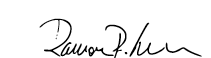
\includegraphics[width=65mm]{figs/logo/assinatura-ramon.png} \\[-4mm]
  \rule[2mm]{70mm}{0.1mm} \\
  \ramon \\[1mm]
  Coordenador do Projeto \\
}

%---------------------------------------------------------------------
\fim